\documentclass{article}

% Language setting
\usepackage[english]{babel}
\usepackage{listings}
\usepackage{xcolor}
\usepackage{float} % Add this line
\usepackage{amsmath}
\usepackage{tikz}
\usepackage[letterpaper,top=2cm,bottom=2cm,left=3cm,right=3cm,marginparwidth=1.75cm]{geometry}
\usepackage{graphicx}
\usepackage[colorlinks=true, allcolors=blue]{hyperref}
\usepackage{titlesec}

% Remove indentation
\setlength{\parindent}{0pt}

% Add space between paragraphs
\setlength{\parskip}{1em} % Adjust the length as needed

% Customizing section titles
\titleformat{\section}{\large\bfseries}{\thesection}{1em}{}
\titleformat{\subsection}{\normalsize\bfseries}{\thesubsection}{1em}{}
\titleformat{\subsubsection}{\small\bfseries}{\thesubsubsection}{1em}{}

% Adjust spacing before and after section titles
\titlespacing*{\section}{0pt}{1em}{0.5em}
\titlespacing*{\subsection}{0pt}{0.8em}{0.4em}
\titlespacing*{\subsubsection}{0pt}{0.6em}{0.3em}
\title{Bitfinity Network: Asynchronous Tokens Enabling Sharding}

\author{Bitfinity Team}

\begin{document}
\maketitle

\begin{abstract}
\noindent The Bitfinity Network introduces a new paradigm for Ethereum Virtual Machine (EVM) computation by integrating EVM processors and asynchronous tokens within a sharded blockchain framework. Utilizing the Internet Computer's dedicated hardware and fast-finality BLS threshold signatures for consensus, Bitfinity achieves impressive throughput and scalability. Each EVM processor can handle hundreds of transactions per second, reaching finality within one to two seconds. Our framework allows tokens to be deployed independently from the EVM, enhancing parallel processing and speed. Moreover, Bitfinity's design enables linear scalability by increasing the number of EVM processors.

Bitfinity also provides a near-native user experience for cross-chain bridging. By incorporating BitFusion and Chain-key Cryptography, Bitfinity functions as a Bitcoin Layer 2 builder and supports the bridging of various assets across multiple chains, as detailed in the BitFusion whitepaper\footnote{BitFusion Briging Paper - 
https://github.com/bitfinity-network/whitepapers/blob/main/BitFusion.pdf}.

\end{abstract}

\tableofcontents

\section{Scaling the EVM through Sharding}
In the discourse on scaling the Ethereum Virtual Machine (EVM), it’s crucial to examine different strategies for parallelization. While traditional EVM-based blockchains operate on a purely sequential model, which inherently limits their scalability to the capacity of a single thread of execution, some blockchain platforms, including SUI\footnote{Sui whitepaper, sections on Move and Narwhal and Tusk consensus - \cite{sui}}, Aptos, and Solana \footnote{Solana white-paper, section on Parallel Merkle Trie - \cite{solana}}, focus on parallelizing computation at the processor level — thereby greatly enhancing scalability but still limiting it to the number of processors available on a single machine.

Moving away from single-threaded execution, other blockchain architectures, such as the Internet Computer, facilitate the asynchronous operation of each smart contract, allowing them to run independently. Rather than opt for the fully asynchronous approach, which limits the atomicity and composability of smart-contracts on the platform, Bitfinity introduces an innovative method to scale, which incorporates both the benefits of asynchronous processes and the safety and composability inherent to synchronous EVM code execution. \footnote{DankSharding - \cite{danksharding}}. 

 The core of this approach involves treating tokens as independent units of concurrency. Under this model, tokens operate as fully independent actors realized as canisters (decentralised web-servers) and are moved just-in-time to EVM canisters, where transactions involving these tokens are processed synchronously; the system implements sharding by separating the state that holds token balances from the instances performing the comuptations.  This hybrid approach leverages the asynchronous actor model \footnote{Internet Computer Blockchain, section on actor model - \cite{icpgeeks}} compute paradigm to enhance scalability without departing from the proven security and stability of the synchronous EVM architecture.

Our methods represent a significant shift in how blockchain technologies manage concurrency and scalability. Rather than rely on a finite number of cores within a single machine, which limits the extent to which parallel processing can be executed, Bitfinity's model enables scaling by adding more EVM instances. Each instance can run decentralized applications (Dapps) independently, thus distributing the workload across multiple EVMs, while maintaining a consistent security model throughout.

In summary, Bitfinity's approach to sharding, which involves treating tokens as independent units of concurrency and processing them within a scalable network of EVM instances, offers a promising solution to the scalability challenges faced by traditional EVM-based blockchains, balancing the needs for scalabale software systems and composable smart-contracts. 


\section{The Bitfinity Network}
\subsection{Network Assumptions}

Bitfinity EVMs are implemented by decentralized canisters, which are powerful smart contracts that communicate with one another according to the constraints of the actor framework. Multiple actors are run by nodes within subnets. The node infrastructure executes messages between these actors, and the subnet collectively reaches consensus on message ordering. Under a partially synchronous communication model,  the communication protocol between nodes on the subnet is Byzantine fault tolerance.

Cross-subnet communication is authenticated using BLS signatures, with the subnet public key created through a key generation protocol. The choice of BLS signatures, known for their efficient aggregation, ensures secure and efficient message validation across subnets. Each subnet operates autonomously, with mechanisms for proactive resharing of secrets to maintain security even when the membership of the subnet changes. Detailed information on the network architecture and assumptions can be found in Appendix Schedule A.

\subsection{Asynchronous Tokens}

Asynchronous tokens on the network adhere to the ICRC-2 standard \footnote{ICRC standard proposals - \cite{icrc}}, incorporating methods such as transfer, approve, and transferFrom. This token standard, modeled on ERC20, is adapted for asynchronous communications. In the current implementation, up to 500 concurrent invocations of these methods can be sent to a canister, with processing completed within a few seconds. Our just-in-time bridging mechanism, which calls these methods, enables Bitfinity tokens to be moved to an EVM subnet in a few seconds.

Messages to a canister that update state are typically finalized within a few seconds, owing to the fast finality of the threshold signature scheme that the subnet uses to reach consensus. As a result of this fast-finality, bridging asynchronous tokens into an EVM environment as ERC-20 \footnote{ERC-20 standard - \cite{erc20}} tokens takes just a few seconds and is seamless (on Ethereum, this would not be possible due to the longer confirmation times).

We refer to this process as \textit{just-in-time bridging}. The process of just-in-time bridging is orchestrated by a specialized bridging canister that facilitates communication between the EVM and the network tokens. When bridging is initiated, tokens are escrowed by the bridge canister. This canister is responsible for minting the corresponding tokens as ERC-20 tokens on the EVM, ensuring interoperability between asynchronous ICRC-2 tokens and synchronous ERC-20 tokens within the EVM while maintaining the scalability and independent operation of each token canister. The workflow for bridging is presented below; see the BitFusion paper for more in-depth coverage\footnote{BitFusion Briging Paper - https://github.com/bitfinity-network/whitepapers/blob/main/BitFusion.pdf}.


\subsection{Just-in-time Bridge Workflow}

\subsubsection{Move ICRC-2 to the EVM}

To transfer ICRC-2 tokens to the EVM, the process involves the following steps:

\begin{enumerate}
\item \textbf{Approve the Bridge Canister}: The user approves the bridge canister to spend their ICRC-2 tokens. This approval also encodes the user's wallet address.
\item \textbf{Call Bridge Smart Contract}: The user calls a bridge smart contract on the EVM, passing their encoded EVM wallet address as an argument. This triggers an event containing the address.
\item \textbf{Event Triggers Mint Transaction}: The event triggers the bridge canister to prepare a mint transaction, minting tokens for the user on the bridge smart contract.
\end{enumerate}

This process is illustrated in Figure \ref{fig
}.

\begin{figure}[H]
\centering
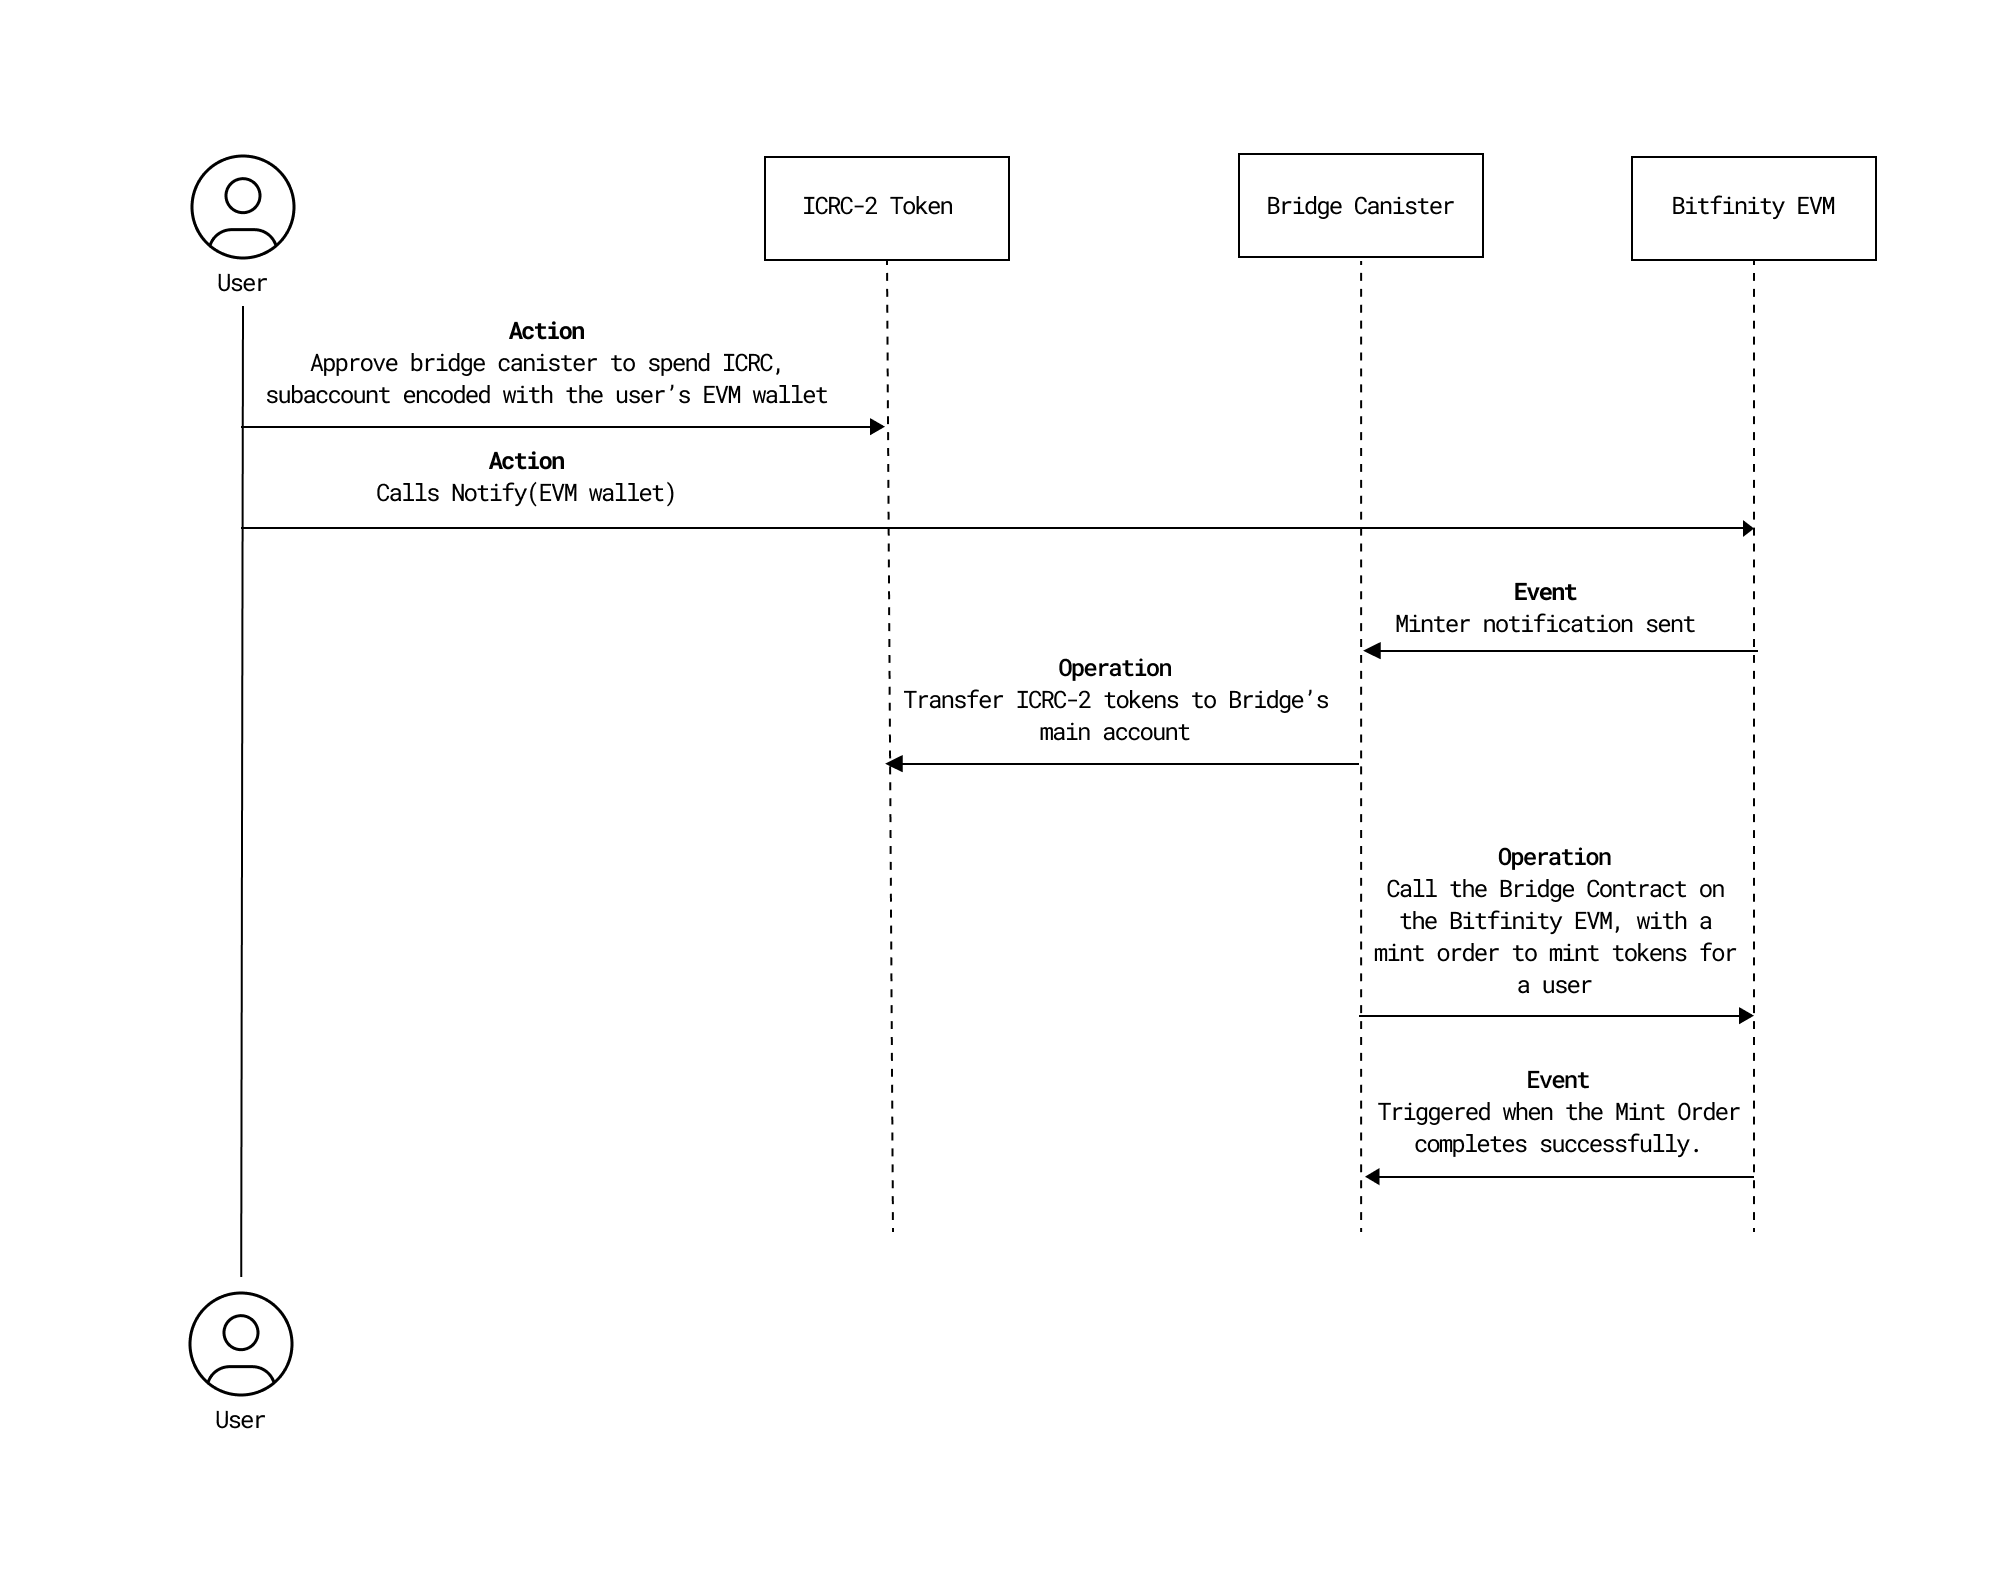
\includegraphics[width=1\linewidth]{icrc-evm.png}
\caption{ICRC-2 to EVM Flow}
\label{fig
}
\end{figure}

\subsubsection{Move ERC20 tokens out of the EVM}

To withdraw ICRC-2 tokens to the EVM, the process involves the following steps:

\begin{enumerate}
\item \textbf{Approve the Bridge}: The user approves the bridge smart-contract on a Bitfinity EVM to spend their bridged ERC-20 tokens.
\item \textbf{Burn ERC-20 Tokens}: The user burns the bridged ERC-20 tokens by calling the burn function on the bridge smart contract, specifying the recipient ICRC-2 address as information to be recorded in the burn event.
\item \textbf{Event Triggers Transfer}: This action emits a burn event on the EVM. The bridge canister polls for this event and, upon receiving it, issues a transfer of ICRC-2 tokens to the recipient as specified by the recipient field of the burn event.
\end{enumerate}

This process is illustrated in Figure \ref{fig
}.

\begin{figure}[H]
\centering
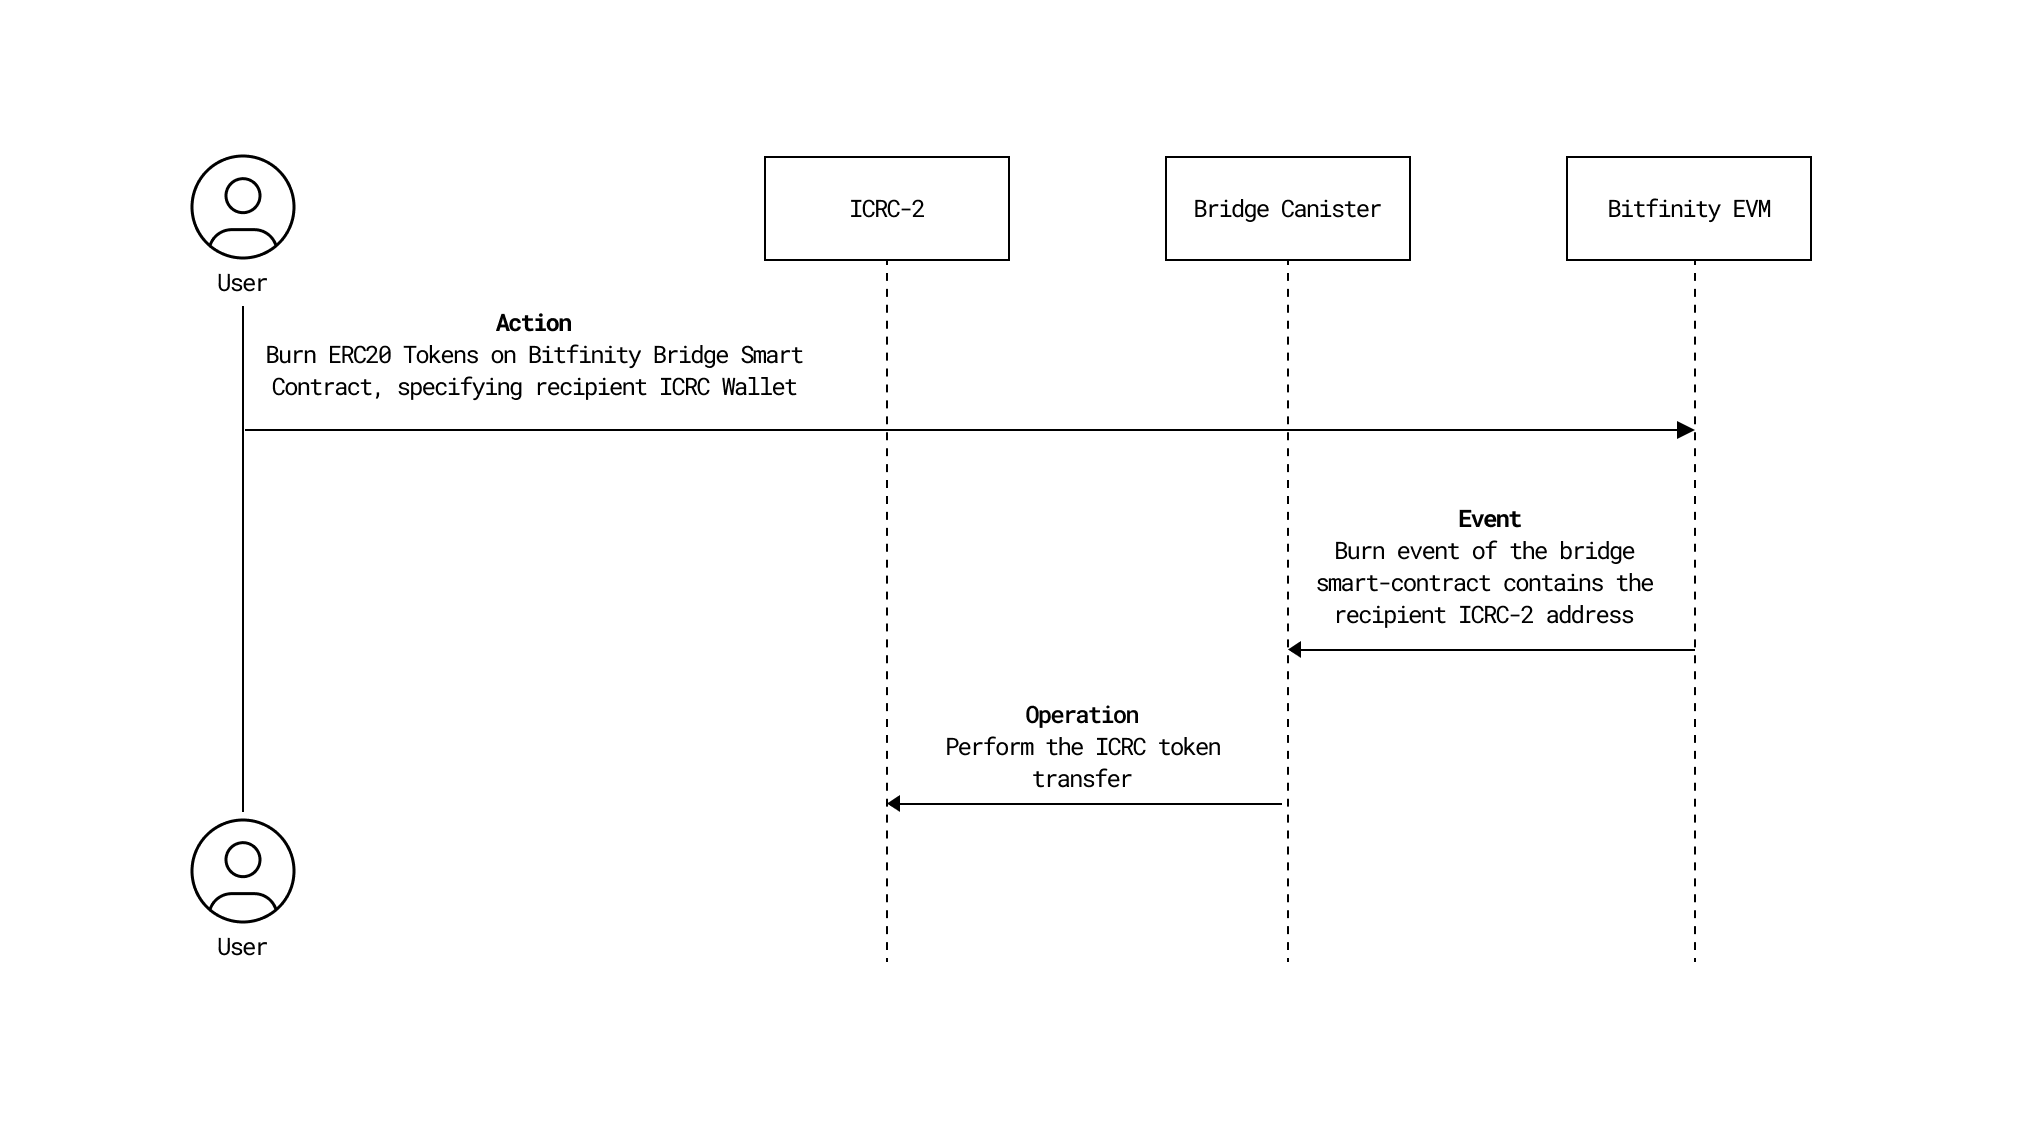
\includegraphics[width=1\linewidth]{evm-icrc.png}
\caption{EVM to ICRC-2 Flow}
\label{fig
}
\end{figure}

\subsubsection{Summary}

The Bitfinity Network scales transaction throughput linearly by sharding the blockchain through separate token and EVM deployments. Bridge canisters ensure efficient, secure communication, enabling just-in-time bridging to EVM instances. This framework is extensible to cross-chain tokens, enhancing interoperability and the bridge UX.

\section {Bitfinity EVM Architecture}
\subsection{Introduction}
In this section we describe the architecture of a Bitfinity EVM in detail. A Bitfinity EVM comprises several essential components, which fall under two broad categories: on-chain and off-chain components.

The on-chain components are responsible for processing transactions and verifying signatures. These components ensure the integrity and security of the blockchain by processing transactions, storing blocks, executing smart-contract byte-code according to the rules of the EVM, and updating the state of the blockchain, which includes both contract and account data authenticated by a Patricia Merkle-Trie.

The off-chain components store blocks and retrieve historical data. These components ensure access to past transactions and other historical information. By managing storage and retrieval tasks, the off-chain components help maintain the availability for blocks removed from the on-chain data storage, and also enable  advanced developer capabilities like running an archive node or debugging the EVM.

\section{On-Chain EVM Components}

At the core of the on-chain architecture there are two canister, the EVM canister and the Signature Verification Canister.  The interactions between these two canisters is described in figure \ref{fig:evm-arch}.

 \begin{figure}[H]
    \centering
    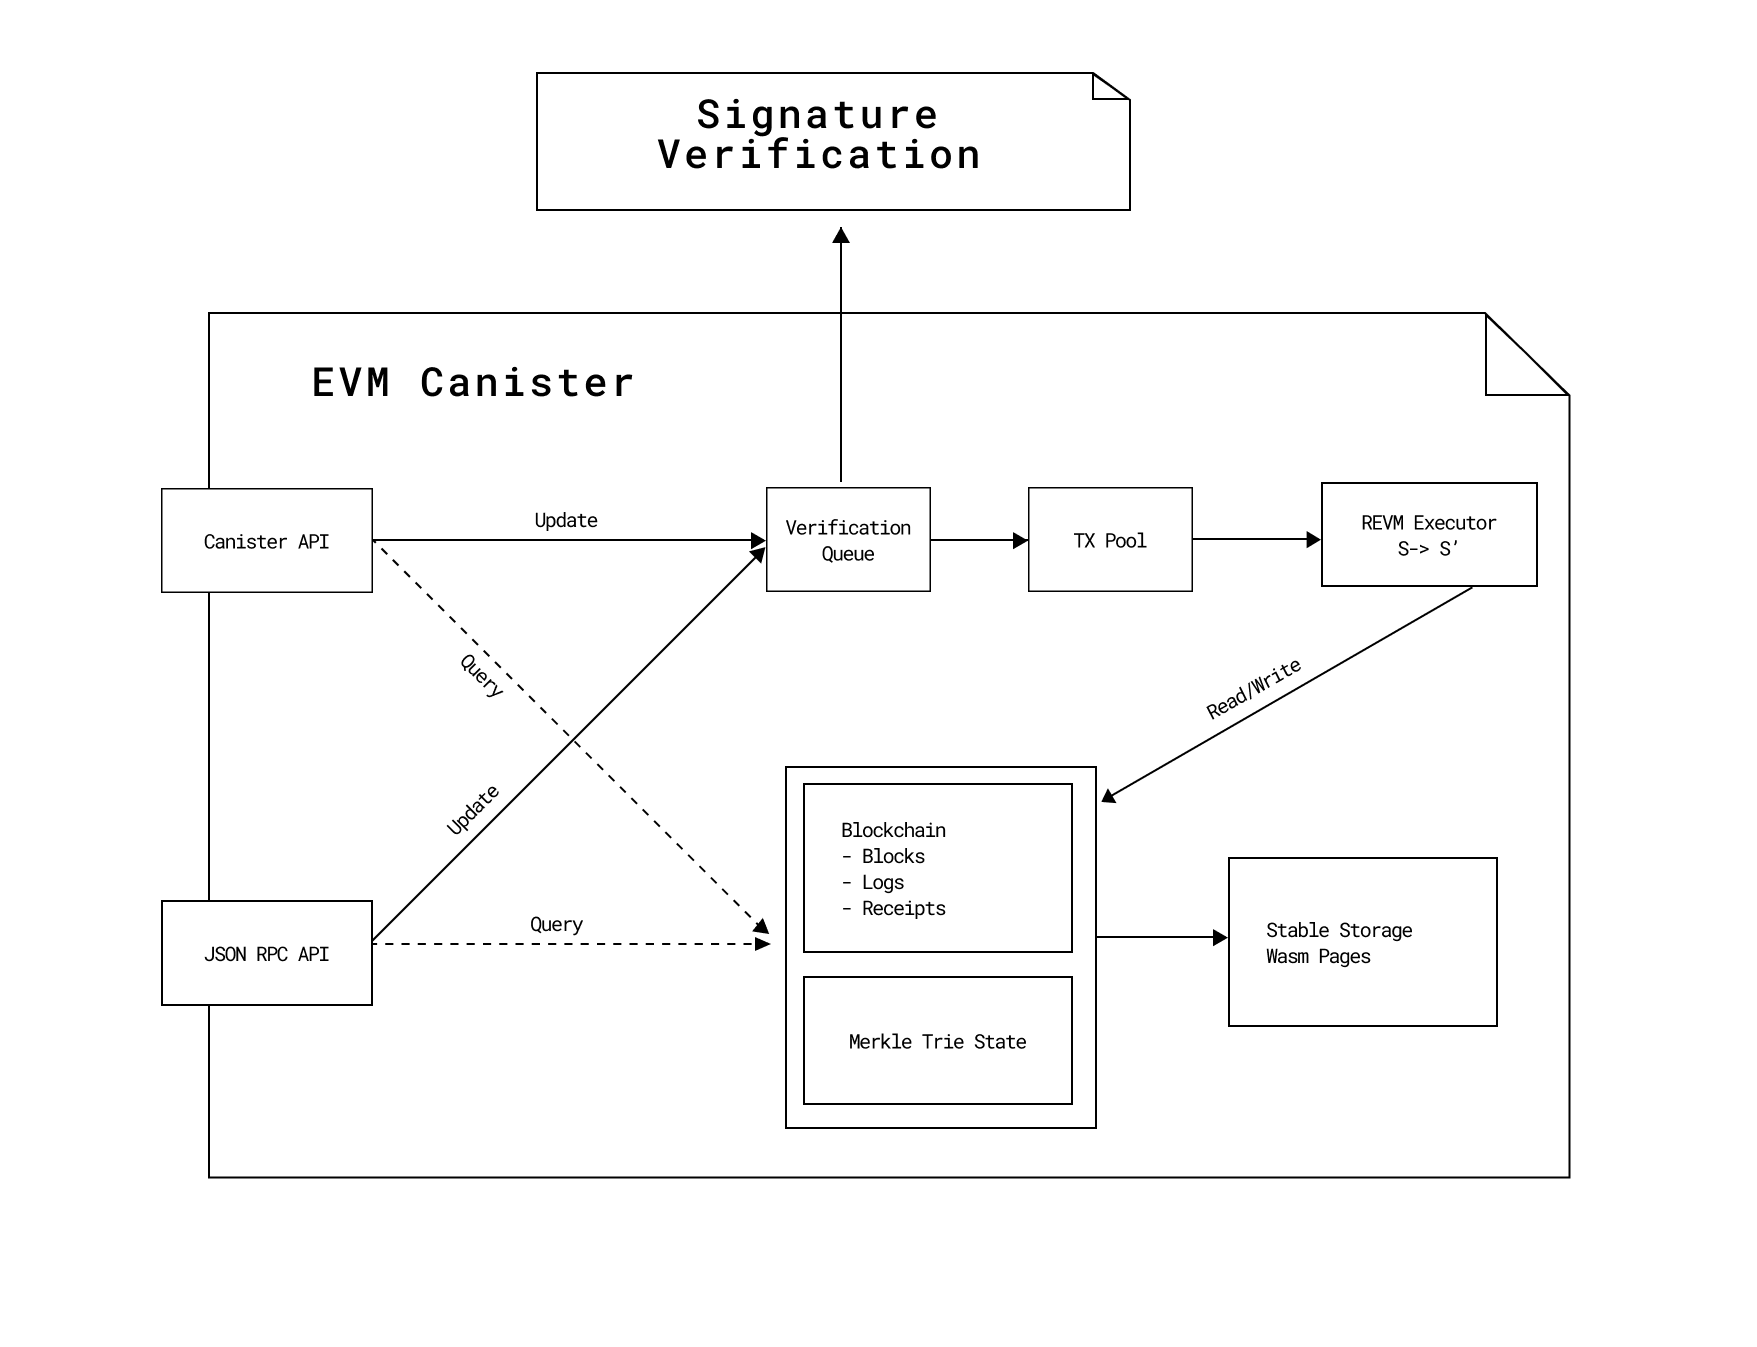
\includegraphics[width=0.9\linewidth]{architecture.png}
    \caption{EVM Architecture}
    \label{fig:evm-arch}
\end{figure}

 The EVM canister serves as the primary entry point for the system and hosts the JSON RPC API through the canister’s HTTP interface. The EVM canister receives transaction requests to this interface from Ethereum clients, such as Metamask wallets; additionally, the canister exposes the same interface to canisters on the network. Upon receiving transactions through either API, the canister pushes transactions into a verification queue. Once the signatures on transactions have been verified and they have passed through the pool, the transactions are then batched to a  block and passed to an REVM-based executor, which executes the block transactions and updates the blockchain state. The blockchain state is maintained within a stable-storage data structure, using an adapted version of Parity’s Merkle Trie \footnote{Parity Technology - \href{https://github.com/paritytech/trie}{Merkle Trie Repo}}, tailored for canister storage (WASM-based). A limited history of blockchain data is retained on this canister, with historical blocks being pruned from storage; these blocks are also accessible via the Ethereum JSON RPC API.

Before a transaction is added to the pool, the Signature Verification Canister verifies the correctness of Ethereum signatures. Given that signature verification is computationally intensive and requires substantial CPU cycles, this task is offloaded to a dedicated canister. This separation of duties optimizes performance and ensures that the main EVM canister remains unburdened by heavy computations.

This architectural design allows the Bitfinity EVM to achieve high efficiency and scalability, supporting robust transaction processing while keeping the on-chain data footprint low. It reduces the need to explicitly run your own EVM nodes or RPC providers to query recent data, as the canister can be queried through the HTTP interface exposed by the network. 

The following sections describe the different components of the EVM canister and the signature verification canister in more detail. For information on the dependencies, see Schedule B of the appendix.  

\subsection{EVM Executor}
The EVM executor is an implementation of the Ethereum Virtual Machine running inside the canister. It consists of code to execute Ethereum transactions, generate blocks and update the state DB, and is based on REVM\footnote{A fast and flexible Rust implementation of the EVM. Refer to \ref{sssec:revm-processor} for more details.}. The executor interfaces with a modified version of Parity's Patricia-Merkle Trie implementation, which updates the canister storage. This storage is based on WASM pages and is accessible through the \textit{stable-storage} API. It serves as the backend for the Merkle Trie's state database, which stores the Merklized Account and Contract data that comprise the state on the EVM.







\subsection{Ethereum JSON RPC API}

The JSON RPC API implements the Ethereum JSON RPC specification which enables the EVM canister to receive requests from external Ethereum libraries (e.g. web3.js), wallets (e.g. Metamask), and other EVM clients. Every time a call is received, the endpoint decodes the content and translates it into a \textit{query} [non-state changing] or an \textit{update} [state-changing] call to be dispatched by the EVM executor. 

Every method of the JSON RPC API has a corresponding network endpoint which allows canisters to interact with the EVM on the network directly, without interfacing with the HTTP gateway. Before a canister can sign transactions on the EVM it must register a public key\footnote{See the \href{https://docs.bitfinity.network/ic-agent/overview}{IC agent docs}} or alternatively use the threshold ECDSA API \footnote{For more details on tECDSA see: \cite{tECDSAprimer}} to sign transactions.  

\subsection{Blockchain Data}
Blockchain Data is a data structure on the EVM that contains the most recent blocks, intended to store at least two weeks of recent block data. Our implementation stores the most recent two weeks of block data, and persists this data to stable-storage. It would be infeasible to store all the blockchain data on-chain, as this could run into terabytes of storage. Instead, we store the full block data on an adapted Reth node. The latest block data includes the Merkle state root, which is then signed, using a BLS threshold signature, by a subnet on the network. These signatures prove to any downstream clients that the block they are interacting with is a part of the cannonical blockchain. As a result of this, syncing the block data from a Bitfinity EVM can be done quickly and trustlessly with much less overhead than on typical proof-of-work EVM networks. 

\subsection{Transaction Pool}

Transaction requests are enqueued in a persistent transaction Pool within the EVM canister. The transactions are then prioritized based on the gas fee and passed from the pool to the EVM Executor.

\subsection{Signature Verification Canister}

The signatures on transactions are verified through the use of a dedicated canister. We use a separate canister  to optimise transaction throughput as verification is relatively computationally expensive and could block the main thread of the EVM canister as it executes transactions.

\section{Off-Chain Components}


Several off-chain services are deployed to ensure redundancy when storing the full block data and to enable the full block data to be queried through the JSON RPC. EVM canisters typically support querying two weeks of block data directly on chain. The off-chain components used within the network are listed as follows:

\begin{itemize}
    \item Block Extractor
    \item Adapted Reth Node
    \item EVM Archiver
\end{itemize}


 To summarise briefly the function of these three services: The Block Extractor is designed to ensure redundancy in data storage. Operating as a Docker daemon, it continuously polls the JSON RPC, requesting blocks which it then stores on a database in the cloud. The  Reth node has been adapted  to ingest blocks from the EVM’s HTTP interface, rather than through the typical P2P interface. It maintains a full history of the EVM data, serves the full JSON RPC API, and can forward transactions to the EVM canister for processing. The EVM-archiver synchronizes with the full state of the EVM canister. Unlike the Reth node, the EVM-archiver operates in an environment similar to the EVM running on a canister, using memory-mapped files as a backend for its WASM-page indexed storage.

The deployments for these separate services can be orchestrated through the use of infrastructure-as-code tools like Terraform, which are open-sourced and made available to the public.

\subsection{Block Extractor}

The Block Extractor is an important off-chain component built to index and store all blockchain data efficiently, given the limitations to storing all this data on chain. Operating as a Docker daemon, the Block Extractor continuously polls the Bitfinity EVM, extracting and processing blocks in real-time. This process involves parsing the blockchain data and storing it on a database in a cloud provider. Multiple instances of the block-extractor are run to ensure redundancy and availability. By maintaining a comprehensive and up-to-date index of all block data, the Block Extractor supports querying for blocks through the JSON RPC API, enabling quick and reliable access to historical data. 

\subsection{Adapted Reth Node}

The adapted Reth node is a full node that ingests blocks from the EVM's HTTP interface or a block-extractor, diverging from the approach that syncs blocks through a typical peer-to-peer network. Our  Reth node implementation maintains a complete history of EVM data, ensuring that all transactional information is preserved and accessible. The node provides a full implementation of the Ethereum JSON RPC API, facilitating seamless interaction with Ethereum-based tools and applications. Additionally, the Reth Node can forward transactions to the EVM canister for processing, integrating tightly with a Bitfinity network EVM. 
To ensure the validity of the synced block data, the Reth node is adapted to verify that the block data has been signed by the subnet, by verifying the BLS signature on the latest block synced. This ensures the block data and state is the same as what was generated by an on-chain Bitfinity EVM. Detailed instructions for building and running the Reth Node can be found in the Bitfinity Developer Documentation \footnote{\href{https://github.com/bitfinity-network/reth/blob/bitfinity-archive-node/bitfinity.md}{Bitfinity Developer Documentation}}. 

\subsection{EVM Archiver}

Unlike the Reth node, the EVM Archiver is primarily used for debugging. It replicates an environment similar to the EVM on a canister, using memory-mapped (MMapped) files which provide a back-end for the WebAssembly (WASM) page interface. This setup allows for accurate local debugging and detailed examination of data structures and values from the main network.

\section{Performance and Competitive Analysis}

A single EVM instance has been benchmarked to achieve between 250 TPS and 1000 TPS, depending on its configuration, and this can be further scaled to a large number of EVM instances. 

In contrast, several Ethereum Virtual Machines (EVMs), such as SEI \footnote{See Sei whitepaper: \cite{sei}}, have adopted parallel processing techniques, achieving speeds up to five times faster than traditional EVM implementations. This performance enhancement is partially constrained by the high frequency of transactions involving the same state. The inherent design of the EVM state storage, which groups and Merklizes the state for each smart contract, limits the extent of parallelism. For instance, transactions involving popular tokens like wETH, which account for approximately 10\% of all transactions, must be processed sequentially. A more efficient approach would be to group state on a per-user basis and move state out of the smart-contract. This would enable more effective parallel processing and reduce the sequential update constraints on frequently used tokens.

This approach is exemplified by blockchains using the Move language, which is designed to minimize shared states within contracts by allowing for state to exist independently of the smart contract acting on it,  and thus allow for higher levels of parallelism. Platforms like Solana, Sui, and Aptos have adopted similar strategies, redesigning token structures to reduce interdependent states. However, these modifications risk losing the inherent advantages and broad adoption of the EVM.


We argue a more practical solution for enhancing EVM performance involves running multiple EVM instances concurrently and sharding tokens, effectively moving the token state into the EVM only when needed. This strategy offers a scalable solution with linear and potentially unlimited scalability, maintaining the advantages of the EVM while enabling enhanced transaction throughput. By employing BLS threshold signatures, EVM processes can communicate efficiently with one another, providing an alternative to Layer2 networks where cross-chain communication is less standardized and more constrained.


\section{Security and Testing}

The code is well-tested, and we aim for high coverage across the core modules. By our estimates, we achieve a coverage of almost 99\% of the EVM code-base. The EVM canister successfully passes all the relevant Ethereum client tests \footnote{see: \href{https://github.com/ethereum/tests}{ethereum/tests}}, currently the gold-standard test-suite for Ethereum node implementations. We also make use of the Parity Tests for our adapted Patricia Merkle-Trie implementation. For more details on our testing and audits please see schedule C of the appendix. 

\section{Conclusion}

The Bitfinity Network has successfully implemented a sharded blockchain leveraging asynchronous tokens and EVM processors, marking a significant advancement in blockchain technology. By treating tokens as independent units of concurrency and utilizing just-in-time bridging mechanisms, Bitfinity enables rapid and efficient transaction processing. Our innovative architecture supports high throughput capable of processing hundreds of transactions per second with finality in just 1-2 seconds, setting a new benchmark for performance. The network is linearly scalable across tokens and EVM. The fast-finality of transfers ensures that just-in-time bridging does not impede user experience (UX).

Through the integration of smart wallets and account abstractions, Bitfinity can ensure seamless token usage across multiple EVM instances. The design of our system allows for interoperability with tokens from other blockchain ecosystems such as BTC, Runes and others, ensuring a better UX for cross-chain applications. By incorporating BitFusion and Chain-key Cryptography, Bitfinity functions as a Bitcoin Layer 2 builder and supports the bridging of various assets across multiple chains, as detailed in the BitFusion paper\footnote{BitFusion Briging Paper - https://github.com/bitfinity-network/whitepapers/blob/main/BitFusion.pdf}.

\nocite*{}
\bibliographystyle{alpha}
\bibliography{sample}

\appendix

\clearpage

\section{Network Architecture and Assumptions}

\subsection{Communication Model}


Bitfinity EVMs run on canisters on subnets provisioned by the Internet Computer (IC) \footnote{Internet Computer - \cite{icpgeeks}}, which employs a partially synchronous communication model to achieve Byzantine fault tolerance, accommodating up to \(f < n/3\) faulty nodes. This model is a practical compromise commonly used in Byzantine fault tolerant systems that do not depend on synchronous communication, as seen in other systems [\cite{castro1999}, \cite{BKM18}]\footnote{See Internet Computer for References - \cite{icpgeeks}}. The partial synchrony allows for certain periods where delays are known but unbounded, unlike purely asynchronous models where delays can be indefinite, often making effective consensus challenging.

In this model, the assumption of partial synchrony specifies that communication between nodes in a subnet alternates between periods of synchrony and asynchronous communication. The system assumes predictable but finite intervals for message delivery, a concept less stringent than the indefinite delays characteristic of fully asynchronous systems (as discussed in \cite{honeybadger2016}). This temporary synchrony is essential for achieving progress in consensus protocols, ensuring the liveness property of the system, but it is not required for maintaining the correctness of consensus (the safety property).  Partial synchrony is likely to be a more appropriate and realistic model for blockchain systems, and gives rise to consensus protocols that are still provably secure and are fast, but not necessarily live, under the assumption of full asynchrony.





\subsection{Cross-Subnet Communication}

The subnet employs an innovative distributed key generation (DKG) protocol for the BLS signature scheme, known as Chain-Key, to authenticate messages. This protocol constructs a public signature-verification key and provides each node with a share of the corresponding secret signing key. After processing a message, the subnet signs the execution results. Each node in the subnet uses its key share to sign the message, and these signatures are then recombined to form the complete signed message.  The protocol is designed to operate effectively under the partial-synchrony communication model, which assumes a degree of asynchronicity and potential Byzantine faults. 

 Each subnet processes messages independently. When a node on one subnet receives a message from another sub-network, the node can validate the signed message by simply validating a digital signature against the public signature-verification key of the originating subnet. The subnetwork  also implements  proactive resharing of secrets at the beginning of each epoch. This process ensures that any new members in a subnet receive an appropriate share of the secret, while nodes that are no longer members lose access to their shares. This approach not only adapts to changes in subnet composition but also guards against potential security breaches from leaked shares, as reshared secrets render old shares obsolete.

A canister is a smart-contract on a subnet, which can be thought of as being modeled by an \textit{actor}: \footnote{Internet Computer, section on execution - \cite{icpgeeks}} the canister processes each input message it receives in a sequential manner based on its input queue. When processing messages and upating the state of the canister, the may trigger further actions, such as sending messages to other canisters. Every message to a canister will receive a guaranteed response and responses are verified efficiently using BLS signatures.

These mechanisms—guaranteed message delivery, threshold signatures, and the robust security model designed for partial synchrony—constitute the key features of the infrastructure that Bitfinity relies on.

\section{EVM Dependencies} 

In building the EVM, we have attempted as far as possible to reuse useful libraries implemented by others. Here we outline some of the useful open-source libraries that have been used. 

\subsection{Parity-Tech's Patricia Merkle Trie}
Bitfinity uses an adapted version of Parity-Tech's Patricia Merkle Trie, which interfaces with a database that interfaces with the stable-storage APIs on the network, where the data is saved to WASM-pages, the backbone of the canister storage.  

\subsection{REVM as an EVM processor} \label{sssec:revm-processor}

\href{https://github.com/bluealloy/revm REVM}{REVM} is a modern EVM written in Rust that is focused on speed, simplicity, compatibility, and stability. REVM is a relatively new project but it passes all the Ethereum Client Tests and, according to our team's benchmarking results, processes transactions nearly twice as fast as GETH, an alternative EVM node implementation, .

\subsection{Bitfinity's Canister SDK}
The Bitfinity EVM is built on top of the Bitfinity \href{https://bitfinity.network/canister-sdk bitfinity-network/canister-sdk}{canister-sdk} and other storage libraries for state management. The canister-SDK provides a streamlined framework for developing canisters, which includes many useful features like unit-testing inter-canister calls, trait-based inheritance as well as libraries for using useful data-structures that use WASM-pages as the underlying storage. 

\subsection{Foundry} Foundry is a  fast, portable, and modular toolkit for Ethereum application development written in Rust, which provides a node, testing framework, and various EVM utilities and types. Bitfinity uses Foundry for testing. 

\clearpage 

\section{Security and Audits}

An initial audit by Quantstamp \footnote{See \href{https://quantstamp.com/}{Quantstamp}} identified 14 high to medium severity issues in the Bitfinity EVM Canister. The development team responded promptly and effectively, resolving all issues. As of November 23, 2023, Quantstamp has verified that all high to medium severity findings have been addressed, with statuses of fixed, acknowledged, or mitigated. Fuzz tests conducted on key components showed no system crashes. 

\subsection{DOS - Attack Vectors and Mitigation}
The network supports three types of method calls to canisters: query, update, and certified queries. Query calls to canisters are non-replicated, with responses issued by a single boundary node. Update calls pass through consensus, achieving network certification with a latency of a few seconds. Certified queries are replicated by multiple boundary nodes, offering reduced latency compared to update calls.

Currently, canisters on the network can handle hundreds of update calls per second, and the network can manage virtually limitless numbers of query and certified query calls. The network infrastructure provides anti-DOS mitigation for query calls. Consequently, the bottleneck in our system lies in ensuring there are no DOS attack vectors against update calls to the JSON RPC interface. To ensure this, we utilize the canister’s inspect message API to prevent users without sufficient balances from calling any state-changing endpoints on the EVM. The inspect message API will block all invalid update calls before they reach consensus, thus mitigating any costly DOS attack.  All state-changing endpoints, such as submitting transactions, must go through the transaction pool, ensuring users are charged the corresponding fee.

\end{document}

